% Figure: second-moment lengths per level for the nearest-neighbor precision on Z (prop:ren-depth), Pi_ii = eps + 2a,
% Pi_{i,i+-1} = -a, with eps/a = 1e-3 and block factor b = 2, in units of the level-l lattice (block units).
% cosh m = 1 + eps/(2a), m = 0.0316215; xi_2 = 1/(2 sinh(m/2)) = (a/eps)^{1/2} = 31.6228; xi_OZ = 1/m = 31.6241.
% Exact law decimated l times (thm:ren-decimation): xi_2^(l) = 1/(2 sinh(b^l m/2)) = 31.62, 15.81, 7.901, 3.942,
% 1.956, 0.9473, 0.4189, 0.1345, 0.01747, 3.050e-4 for l = 0..9 (9.30e-8 at l = 10, off the axis).
% Coarse (Galerkin) medium of blocks of side b^l (prop:ren-depth(d), equality for nearest-neighbor couplings):
% xi^(l) = xi_2 b^{-l/2} = 31.62, 22.36, 15.81, ..., 0.9882, 0.6988, 0.4941 for l = 0..12.
% Dotted: xi_OZ b^{-l}, the upper bound of prop:ren-depth(b) on the decimated length.
% Dashed: thresholds of prop:ren-depth(a) with D = 1, xi >= (1/2)(r_0 - 1)^{1/2} = 1/2 (r_0 = 2) and 1 (r_0 = 5).
% Last levels on or above them: decimated l = 5 (b^l = 32, r_0 = 2) and l = 4 (b^l = 16, r_0 = 5), within the bounds
% b^l <= (2/m) arcsinh((r_0 - 1)^{-1/2}) = 55.75 and 30.44 of (b); coarse medium l = 11 (b^l = 2048) and l = 9
% (b^l = 512), within b^l <= 4 D xi_2^2/(r_0 - 1) = 4000 and 1000 of (d).
% Cross-checks in double precision: the covariance of the ring of 16384 sites, from its symbol by Fourier inversion and
% subsampled at stride 2^l, gives xi_2^(l) on the covariance side and on the precision side to 1.3e-8 relative for
% l <= 8, with decimated couplings beyond range one below 3e-14; block sums of Pi over 2^l sites, taken directly and
% iterated with b = 2, give coarse leak 2^l eps, range one and xi_2^2/b^l to 3.4e-13 relative.
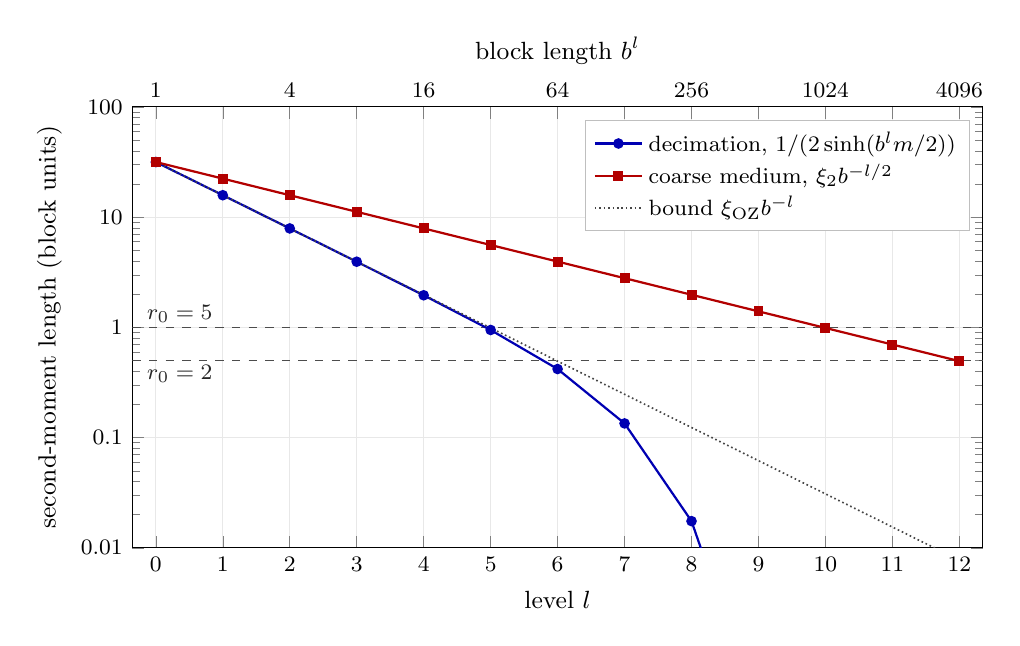
\begin{tikzpicture}
  \begin{semilogyaxis}[name=len, width=10.8cm, height=5.6cm, scale only axis,
      xmin=-0.35, xmax=12.35, ymin=0.01, ymax=100,
      xtick={0,...,12}, ytick={0.01,0.1,1,10,100}, log ticks with fixed point,
      grid=major, grid style={gray!18},
      xlabel={level $l$}, ylabel={second-moment length (block units)},
      every axis label/.style={font=\small}, tick label style={font=\footnotesize},
      legend style={font=\footnotesize, at={(0.985,0.97)}, anchor=north east, draw=gray!50, fill=white,
        cells={anchor=west}, row sep=-1pt}]
    \draw[gray!60!black, dashed] (axis cs:-0.35,1) -- (axis cs:12.35,1);
    \draw[gray!60!black, dashed] (axis cs:-0.35,0.5) -- (axis cs:12.35,0.5);
    \addplot[blue!70!black, thick, mark=*, mark size=1.5pt] coordinates {(0,31.6228) (1,15.8094) (2,7.90076)
      (3,3.94249) (4,1.95558) (5,0.947317) (6,0.418891) (7,0.134505) (8,0.0174705) (9,0.000305032)};
    \addlegendentry{decimation, $1/(2\sinh(b^lm/2))$}
    \addplot[red!70!black, thick, mark=square*, mark size=1.4pt] coordinates {(0,31.6228) (1,22.3607) (2,15.8114)
      (3,11.1803) (4,7.90569) (5,5.59017) (6,3.95285) (7,2.79508) (8,1.97642) (9,1.39754) (10,0.988212)
      (11,0.698771) (12,0.494106)};
    \addlegendentry{coarse medium, $\xi_2b^{-l/2}$}
    \addplot[gray!55!black, densely dotted, semithick] coordinates {(0,31.6241) (1,15.812) (2,7.90602) (3,3.95301)
      (4,1.97651) (5,0.988253) (6,0.494126) (7,0.247063) (8,0.123532) (9,0.0617658) (10,0.0308829)
      (11,0.0154415) (12,0.00772073)};
    \addlegendentry{bound $\xi_{\mathrm{OZ}}b^{-l}$}
    \node[font=\footnotesize, gray!30!black, anchor=south west, inner sep=1.5pt] at (axis cs:-0.2,1) {$r_0=5$};
    \node[font=\footnotesize, gray!30!black, anchor=north west, inner sep=1.5pt] at (axis cs:-0.2,0.5) {$r_0=2$};
  \end{semilogyaxis}
  \begin{axis}[at={(len.south west)}, anchor=south west, width=10.8cm, height=5.6cm, scale only axis,
      xmin=-0.35, xmax=12.35, ymin=0, ymax=1, axis x line*=top, axis y line=none,
      xtick={0,2,...,12}, xticklabels={$1$,$4$,$16$,$64$,$256$,$1024$,$4096$},
      xlabel={block length $b^l$},
      every axis label/.style={font=\small}, tick label style={font=\footnotesize}]
  \end{axis}
\end{tikzpicture}
